\section{Technologien}

\subsection{Software Defined Access (SDA)}
Cisco bietet mit SDA eine automatisierte End-to-End-Segmentierung um den Benutzer-, Geräte- und Anwendungsverkehr zu trennen, ohne das Netzwerk neu zu gestalten. Durch diesen automatisierten Benutzerzugriff ermöglicht SDA Einrichtungen innert kürzester Zeit. Durch diese enorme Vereinfachung wird eine zusätzliche Sicherheit und Skalierung des Betriebs gewonnen. Ebenso wird die Transparenz deutlich erhöht und die schnelle Bereitstellung neuer Dienste gewährleistet. Durch die Automatisierung von täglichen Aufgaben wie Konfiguration, Bereitstellung und Troubleshooting reduziert SDA die Zeit für Netzwerkanpassungen, verbessert die Problemlösungszeit und reduziert die Auswirkungen von Sicherheitsverletzungen.\\
\\
So können Organisationen sicherstellen, dass für jeden Benutzer oder jedes Gerät mit jeder Anwendung die richtigen Richtlinien festgelegt werden über das Netzwerk. Dies wird mit einer einzigen Netzwerkstruktur über LAN und WLAN erreicht, wodurch ein konsistente Benutzererfahrung überall ohne Kompromisse bei der Sicherheit. \\
\\
SDA wird aus mehreren Komponenten zusammengesetzt. Dazu gehört das DNA-Center, welches die grundsätzliche Funktion des Netzwerks sicherstellt, sowie Identity Service Engine (ISE), welches die Benutzeridentitäten und Profile verwaltet.

\subsubsection{Campus Fabric}
Die Fabric bildet ein Overlay Netz. Das Overlay Netz bildet eine virtuelle Topologie um Geräte miteinander zu verbinden, welches auf einer beliebigen physischen Underlay Topologie aufgebaut ist. Das Overlay Netzwerk verwendet oft alternative Weiterleitungsattribute, um zusätzliche Dienste bereitzustellen, die nicht vom Underlay Netzwerk bereitgestellt werden.
\begin{figure}[H]
	\centering
	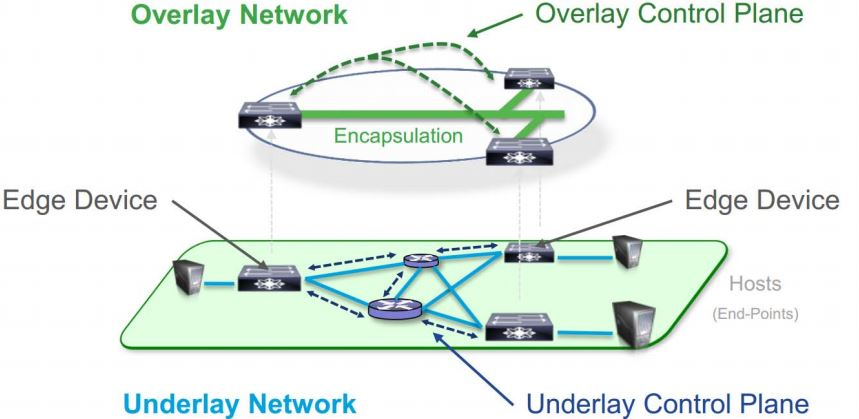
\includegraphics[height=6cm]{img/campusfabric.jpg}
	\caption{Campus Fabric}
	\label{fig:Campus Fabric}
\end{figure}

\subsection{Cisco Digital Network Architecture Center (Cisco DNA-Center)}
DNA Center ist das zentrale Überwachungs-Dashboard für Netzwerke, mit dem alle Cisco DNA-Produkte und -Lösungen verwaltet werden können.
DNA Center gibt die Möglichkeit unter einem Grafischen Nutzer Interface direkt mit APIC(Application Policy Infrastructure Controller)-EM 2.x Applikationen mit der Identity Services Engine (ISE) und mit Network Data Plattform (NDP) unserer Assurance und Analytics Plattform zu sprechen. Alle Parameter die angezeigt oder konfiguriert werden müssen kann man unter DNA Center ausführen und muss nicht zwischen den einzelnen Modulen und Oberflächen hin und her springen.
\begin{figure}[H]
	\centering
	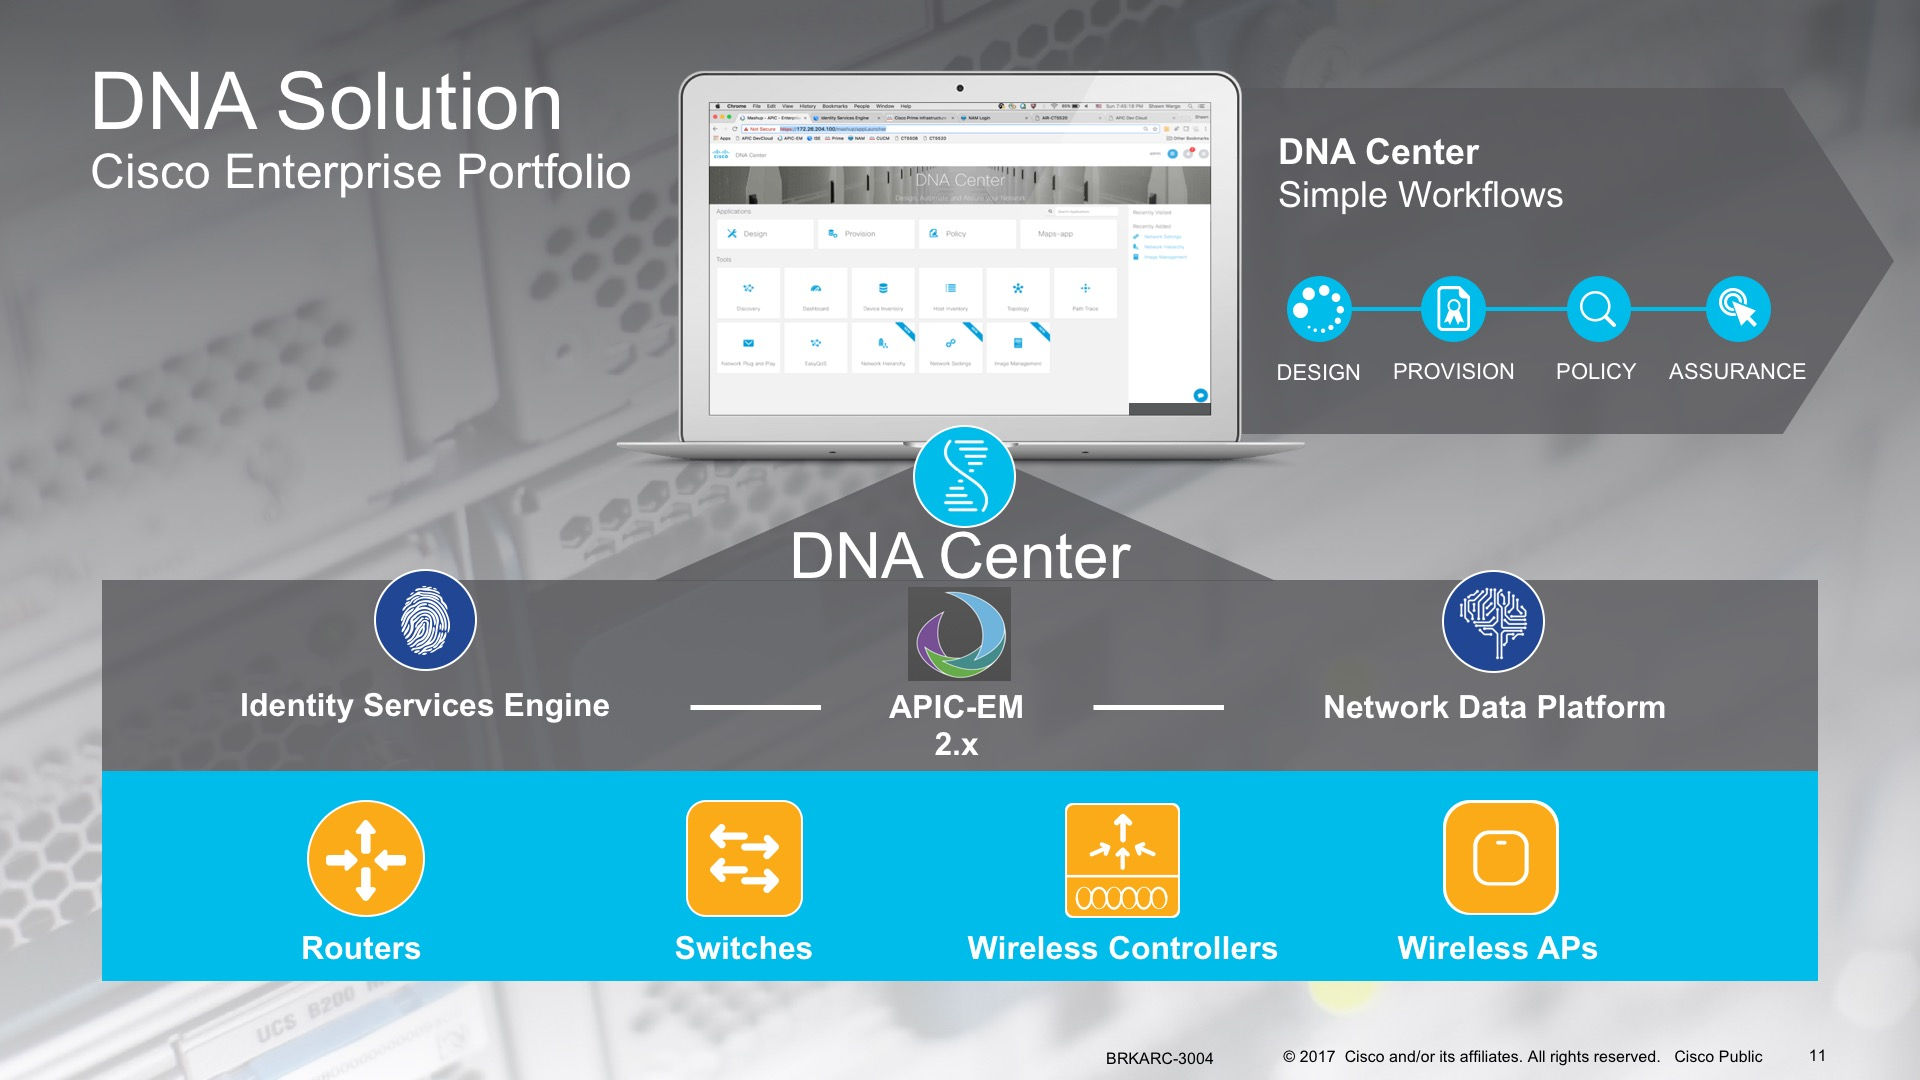
\includegraphics[height=8cm]{img/DNAC-1.jpg}
	\caption{DNA Solution}
	\label{fig:Aufbau einer DNA Solution}
\end{figure}
APIC-EM 2.x automatisiert dann die notwendigen Konfigurationen und spricht mit dem Netzwerk. Auch die Integration von IP Address Management Lösungen wie zB Infoblox werden nur über die DNA Center Oberfläche konfiguriert. \\
\\
SD-Access ist die Grundlage von Cisco DNA. Es ermöglicht Netzwerkzugriff in Minuten für jeden Benutzer oder jedes Gerät für jede Anwendung, ohne Kompromisse. Bei SD-Access folgen die festgelegten Richtlinien automatisch dem Benutzer über alle Netzwerkdomänen hinweg.

\subsection{Identity Service Engine (ISE)}

\subsection{Slack}

\subsection{Locator ID Separation Protocol (LISP)}
LISP ist das Produkt einer Arbeitsgruppe in der Internet Engineering Taskforce (IETF), um was wachsende Problem des doppelten Verwendungszwecks der IP-Adressen zu bereinigen. Zur Zeit wird die IP-Adresse benutzt um die Identität eines Hosts festzulegen und auch den Ort zu bestimmen, an dem er sich im Internet befindet. Dies hat zur Folge das sich bei einem Aufenthalsortwechsel auch die IP-Adresse des Hosts ändert, was bedeutet das die Identität verloren geht und die alten IP-Verbindungen verfallen. \\

Dies soll nun durch LISP geändert werden, in dem es die Identität eines Gerätes, auch Endpoint Identifier (EID) genannt, von seinem Aufenthaltsort, auch Routing Locator (RLOC) genannt, in zwei separate Adressräume unterteilt. Das bedeutet, dass die Router in einer LISP-Architektur nur Routing-Informationen von RLOCs speichern müssen. Um Pfadinformationen eines Hosts abzurufen, kann der Router diese beim LISP-Mapping-Server abfragen, was analog wie das DNS-Mapping funktioniert. \\

LISP verwendet für SDA/Fabric eine VXLAN-Kapselung.

\begin{table}[H]
	\rowcolors{2}{gray!25}{white}
	\centering
	\begin{tabularx}{\textwidth}{p{6.6cm} | X}
		\rowcolor{gray!50}
		\textbf{LISP Device} & \textbf{Function} \\
		\hline	
		ALT (Alternative Logical Topology) & Collects EID data from Map Servers (MS) and advertise aggregate EID prefix. In a deployment of multiple Map Servers, it keeps all synchronized. \\
		
		ETR (Egress Tunnel Router) and PETR (Proxy ETR) & Connects a LISP capable core network. Registers EID prefices with Map Server (MS). Decapsulates LISP packets, received from LISP core. Responds to Map-request messages with a Map-Reply by giving appropriate EID prefix. Typically, this is a CPE (customer premise equipment) router. PETR works on behalf on non-LISP domain and provides LISP-non-LISP connectivity. \\ 
		
		ITR (Ingress Tunnel Router) and PITR (Proxy Ingress Tunnel Router) & Responsible for forwarding local traffic to external destinations. Resolves RLOC for a given destination by sending Map-request to Map Resolver. Encapsulates (vxlan) traffic with LISP header. Typically, this is a Access Layer Switch. PITR works on behalf on non-LISP domain and provides LISP-non-LISP connectivity. \\
		
		XTR (X Tunnel Router) & When both ITR and ETR functions are handled by one router, it is called XTR. This is typical in practice. \\
		
		MR (Map Resolver) & Responds to Map-requests from ITR. Map-requests will be replied with a Negative Map-Reply or forwarded to appropriate ETR or ALT. \\
		
		MS (Map Server) & Registers EID space upon receiving Map-register messages from ETR. Updates ALT and MR with EID and RLOC data. \\
		
		MSMR (Map Server Map Reloader) & When a device acts as both Map Server and Map Resolver, it is called MSMR. This is typical in practice. \\
		
		EID (Endpoint ID) & Endpoint Identifier. IP addresses hidden from core network routing table. RLOC acts next-hop to reach EID space. \\
		
		RLOC (Routing Locator) & Routing Locator. Exists in global routing tables. Authoritative to reach EID space. \\
		
	\end{tabularx}
	\caption{LISP Elements}
	\label{tab:my-label}
\end{table}

\subsection{Virtual Extensible LAN (VXLAN)}
VXLAN ist ein Encapsulation-Protokoll, um ein Overlay-Netzwerk auf einer existierenden Layer 3 Infrasturktur laufen zu lassen. VXLAN wurde ursprünglich von Cisco Systems, VMware und Arista Network entwickelt und ist einer der IETF festgelegten Standards (RFC 7348). \\
\\
Technisch gesehen erzeugt ein VXLAN logische Layer 2 Netzwerke, die dann in standardmässige Layer 3 Pakete eingepackt werden. VXLAN dient dazu um in sehr grossen Netzwerkumgebung die Probleme zu lösen, die durch beschränkte Anzahl von VLANS betroffen sind. Mit VXLAN sind insgesamt 16’777’215 (24 Bit) Layer-2-Umgebungen möglich, die ihrerseits wieder jeweils 4096 VLANs beinhalten können.
